% ==============================================================================================
\section{Results}
\label{sec:results}

All results in this section come from the six lab PCs with rotating rounds. Tables not marked otherwise are from the overnight series on the overnight build, 5 runs per cell; results from the final build are marked. Section~\ref{sec:method} describes how the runs were made and counted.

\begin{table}[!htb]
\centering\small
\caption{Every run, in total.}
\label{tab:totals}
\begin{tabular}{@{}lrr@{}}
\toprule
 & Overnight series & Kill runs (final build) \\
\midrule
Runs & 157 & 49 \\
Requests sent & 199,481,205 & 50,587,740 \\
Answered & 199,464,878 & 48,331,376 \\
Gave up after all retries & 16,327 & 2,256,364 \\
Unaccounted for & 0 & 0 \\
Digest checkpoints compared & 69,715 & 14,932 \\
Digest mismatches & 0 & 0 \\
\bottomrule
\end{tabular}
\end{table}

``Gave up'' is not a failure of the system above what the nodes left can carry: with one node left there is about a third of the capacity, and with none, nobody can answer. The checks that must always hold are 0 unaccounted and 0 digest mismatches.

\subsection{Load balancing: scenarios 1 and 2}
\label{sec:lb}

\textbf{Scenario 1, load changing.} Five runs of 240 s: 1,000 reports a second, then 5,000, then 9,000, then back to 1,000, from all three client PCs, with planning work 1000. Every node kept winning at every load, each between 31.4\% and 34.5\% (Table~\ref{tab:s1}, Figure~\ref{fig:s1}). The bids followed the load, from an expected wait of about 4,400 $\mu$s to about 56,000 $\mu$s and back. Since the PCs are the same model and the load is even, even shares are the fair result. The winner is chosen again for every report, so this is not nodes taking turns. Scenario 2 shows what happens when one node really is busier.

\begin{table}[!htb]
\centering\small
\caption{Scenario 1: share of reports each node won, and its mean bid in $\mu$s of expected wait.}
\label{tab:s1}
\begin{tabular}{@{}lrrrrrrr@{}}
\toprule
Load & Answers/s & Node 1 & Node 2 & Node 3 & Bid 1 & Bid 2 & Bid 3 \\
\midrule
1,000/s & 999 & 33.8\% & 33.1\% & 33.2\% & 4,390 & 4,390 & 4,402 \\
5,000/s & 4,998 & 34.5\% & 31.9\% & 33.6\% & 24,019 & 24,255 & 23,969 \\
9,000/s & 8,998 & 34.2\% & 31.4\% & 34.4\% & 55,891 & 56,554 & 55,863 \\
back to 1,000/s & 999 & 33.7\% & 33.1\% & 33.1\% & 4,410 & 4,427 & 4,452 \\
\bottomrule
\end{tabular}
\end{table}

\begin{figure}[!htb]
\centering
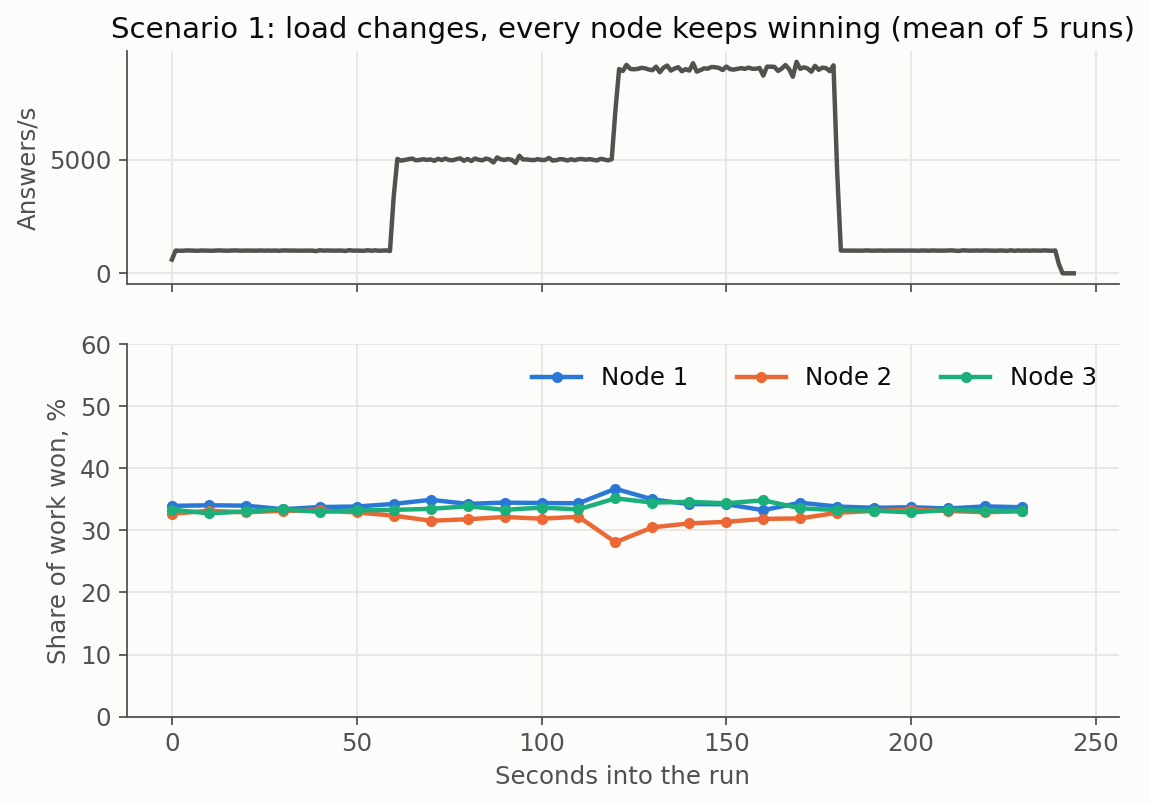
\includegraphics[width=0.82\linewidth]{figures/scenario1.png}
\caption{Scenario 1: shares and bids as the load steps up and down, mean of 5 runs.}
\label{fig:s1}
\end{figure}

\textbf{Scenario 2, one node made slow.} Five runs of 180 s at 3,000 reports a second. From 60 s to 120 s one node's planning work goes from 1000 to 5000, so a plan takes about 20 ms instead of 4 ms; the slowed node changes between runs. The system's score, expected wait, is compared with a queue-only score and with a control run where nothing is slowed (Table~\ref{tab:s2}, Figure~\ref{fig:s2}).

\begin{table}[!htb]
\centering\small
\caption{Scenario 2: share of the slowed node and its bid, before, during and after the slowdown.}
\label{tab:s2}
\begin{tabular}{@{}llrrrr@{}}
\toprule
Score & Phase & Slowed node won & Each other node & Slowed node's bid & Others' bid \\
\midrule
Expected wait (in use) & before & 33.4\% & 33.3\% & 13,831 & 13,791 \\
 & slowed & \textbf{4.9\%} & 47.6\% & 30,393 & 17,883 \\
 & after & 33.3\% & 33.3\% & 13,980 & 13,963 \\
Queue length only & before & 33.5\% & 33.3\% & 88 & 88 \\
 & slowed & 25.2\% & 37.4\% & 93 & 94 \\
 & after & 33.6\% & 33.2\% & 88 & 88 \\
Control, nothing slowed & slowed & 34.7\% & 32.7\% & 13,852 & 13,912 \\
\bottomrule
\end{tabular}
\end{table}

\begin{figure}[!htb]
\centering
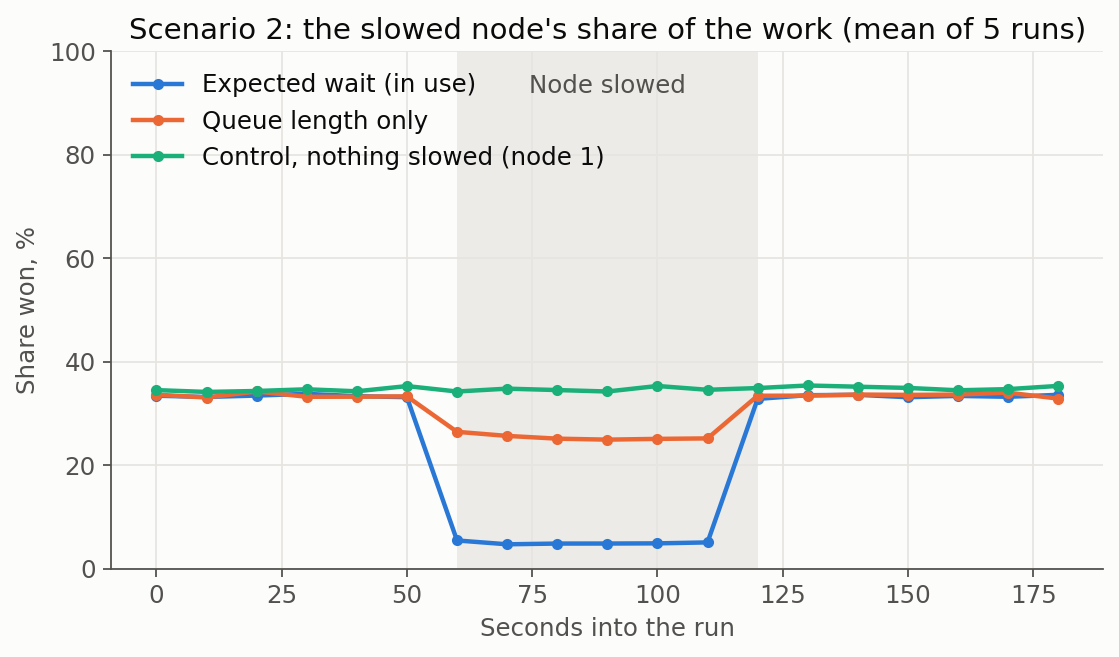
\includegraphics[width=0.82\linewidth]{figures/scenario2.png}
\caption{Scenario 2: the slowed node's share, under the expected-wait score, a queue-only score and the control.}
\label{fig:s2}
\end{figure}

When one node is slowed, its bid more than doubles and its share falls from 33.4\% to 4.9\%, while each of the others takes 47.6\%. When the slowdown ends it is back at 33.3\%. Service does not suffer: the median latency was 136 ms, the same as the control, and nobody gave up. A queue-only score reacts far less, to 25.2\%, because its bids hardly change (93 against 94): at this load a slow plan does not show up in the queue. This is the measured reason for using expected wait.

\subsection{Server failure: scenario 3}
\label{sec:s3}

A node stops answering for 20 s, 45 s into a 150 s run, under load from all three client PCs. The victim changes between runs. Table~\ref{tab:s3} and Figure~\ref{fig:s3} show the results at six loads.

\begin{table}[!htb]
\centering\small
\caption{Scenario 3: a 20 s fault under load, 5 runs per row. ``Dropped'' is when the others went on without the node. The in-flight columns count the reports the silent node had won in its last second: how many were still unanswered 0.3 s after the fault, how many of those the others planned again, and how many already had the silent node's plan in the log.}
\label{tab:s3}
\footnotesize\setlength{\tabcolsep}{4.5pt}
\begin{tabular}{@{}rrrrrrrrr@{}}
\toprule
Offered/s & Planning work & Answers/s during & p99 during, ms & Dropped, ms & Unanswered & Replanned & In log & Gave up \\
\midrule
1,000 & 1000 & 999 & 942 & 1,037 & 23 & 12 & 11 & 0 \\
5,000 & 1000 & 5,005 & 1,535 & 1,043 & 117 & 42 & 75 & 0 \\
8,000 & 1000 & 8,007 & 1,624 & 1,036 & 297 & 82 & 215 & 0 \\
10,000 & 0 & 10,002 & 2,075 & 1,048 & 405 & 23 & 382 & 0 \\
20,000 & 0 & 20,022 & 2,381 & 1,065 & 669 & 9 & 660 & 0 \\
30,000 & 0 & 29,992 & 2,688 & 1,054 & 1,772 & 47 & 1,725 & 12,303 \\
\bottomrule
\end{tabular}
\end{table}

\begin{figure}[!htb]
\centering
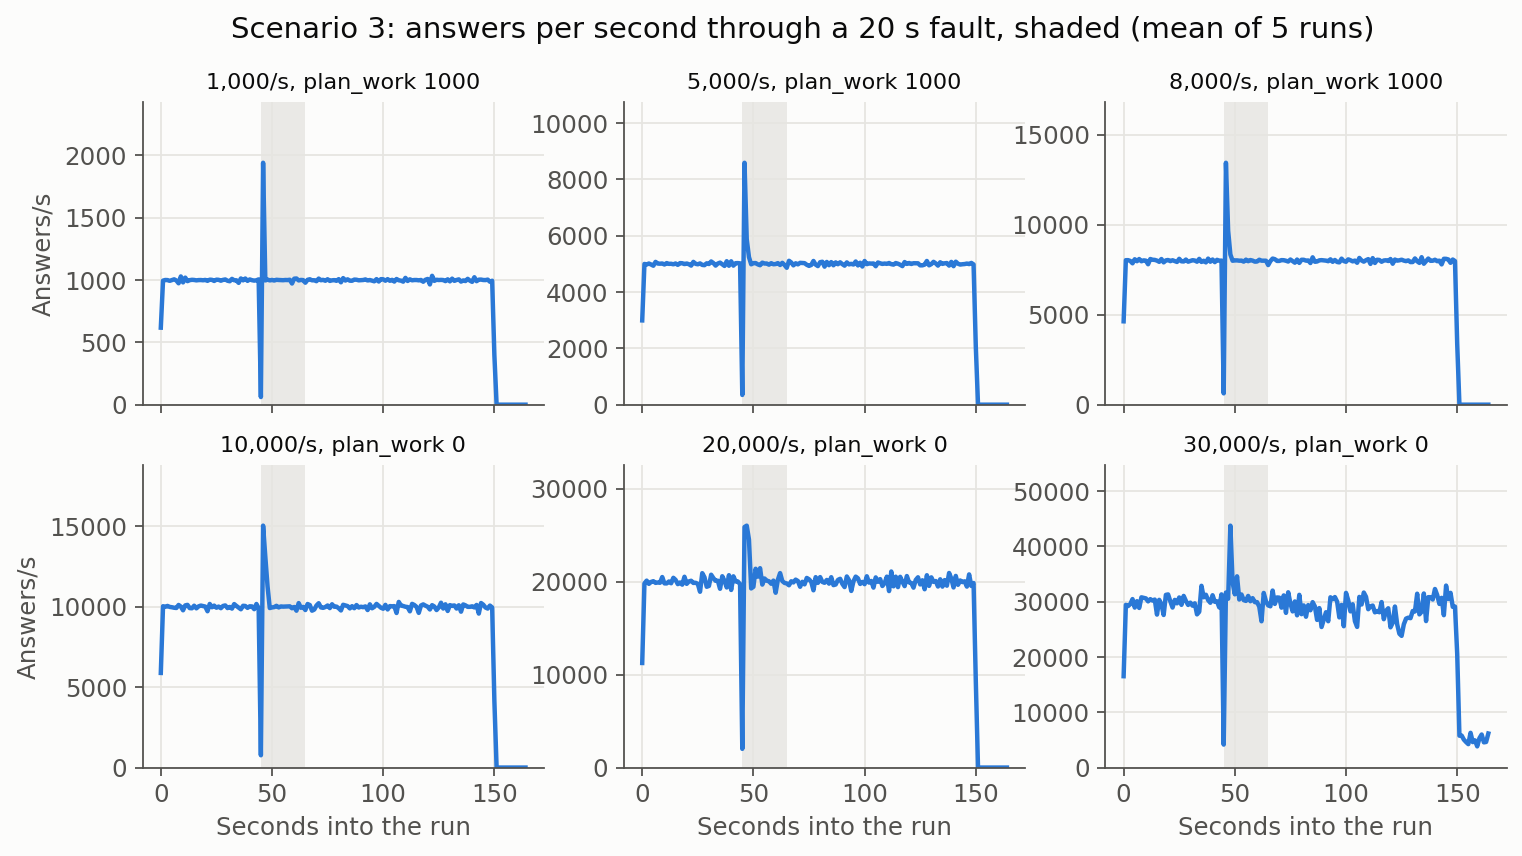
\includegraphics[width=0.9\linewidth]{figures/scenario3.png}
\caption{Scenario 3: answers per second through a 20 s fault (shaded), mean of 5 runs.}
\label{fig:s3}
\end{figure}

\begin{itemize}
  \item \textbf{Failover time} was about 1.04 s at every load, from 1,036 ms to 1,065 ms. It is the detection time, and it does not grow with load.
  \item \textbf{During the fault}, answers fall almost to nothing for about a second, then a burst clears the backlog, and the rate stays at the offered rate for the rest of the fault. The burst is why the ``during'' column equals the offered rate, and the reports caught in that second are why p99 rises.
  \item \textbf{Requests in flight} were all accounted for. Of the reports the silent node had won in its last second, most were answered before it stopped. Of those still unanswered 0.3 s later, at 10,000 a second, 23 were planned again by the others, and 382 already had the silent node's result in the log, so a peer gave that answer.
  \item \textbf{Transparency.} Across 6,879,602 answers given from 2 s into a fault to its end, none came from the silent node. Clients were not told of any failure, and needed no change.
  \item \textbf{The limit.} At 30,000 a second the system is at its edge: in 2 of 5 runs reports gave up, 12,233 and 70.
\end{itemize}

\subsection{Server recovery: scenario 4}
\label{sec:s4}

The same runs give the recovery of the returning node, together with a 5 s fault at 10,000 a second and runs where the process was killed and started 30 s later (Table~\ref{tab:s4}, Figure~\ref{fig:s4}). ``Caught up'' is when it had applied the whole log; ``member again'' is when its proposals were accepted again, which ends recovery.

\begin{table}[!htb]
\centering\small
\caption{Scenario 4: recovery and convergence, 5 runs per row, mean $\pm$ 95\% interval.}
\label{tab:s4}
\begin{tabular}{@{}lrrrrr@{}}
\toprule
Fault, load & Planning work & Caught up, ms & Member again, ms & Mismatches & One digest at the end \\
\midrule
20 s, 1,000/s & 1000 & 290 $\pm$ 73 & 800 $\pm$ 75 & 0 & 5 of 5 \\
20 s, 5,000/s & 1000 & 1,247 $\pm$ 319 & 1,820 $\pm$ 364 & 0 & 5 of 5 \\
20 s, 8,000/s & 1000 & 2,078 $\pm$ 557 & 2,848 $\pm$ 733 & 0 & 5 of 5 \\
20 s, 10,000/s & 0 & 2,801 $\pm$ 637 & 3,632 $\pm$ 809 & 0 & 5 of 5 \\
20 s, 20,000/s & 0 & 6,744 $\pm$ 1,628 & 10,488 $\pm$ 4,118 & 0 & 5 of 5 \\
20 s, 30,000/s & 0 & 14,384 $\pm$ 3,246 & 73,320 $\pm$ 34,451 & 0 & 5 of 5 \\
5 s, 10,000/s & 0 & 875 $\pm$ 162 & 1,414 $\pm$ 199 & 0 & 5 of 5 \\
killed, 5,000/s & 1000 & 6,023 $\pm$ 1,328 & 6,000 $\pm$ 1,324 & 0 & 5 of 5 \\
killed, 10,000/s & 0 & 11,994 $\pm$ 3,219 & 11,958 $\pm$ 3,235 & 0 & 5 of 5 \\
\bottomrule
\end{tabular}
\end{table}

\begin{figure}[!htb]
\centering
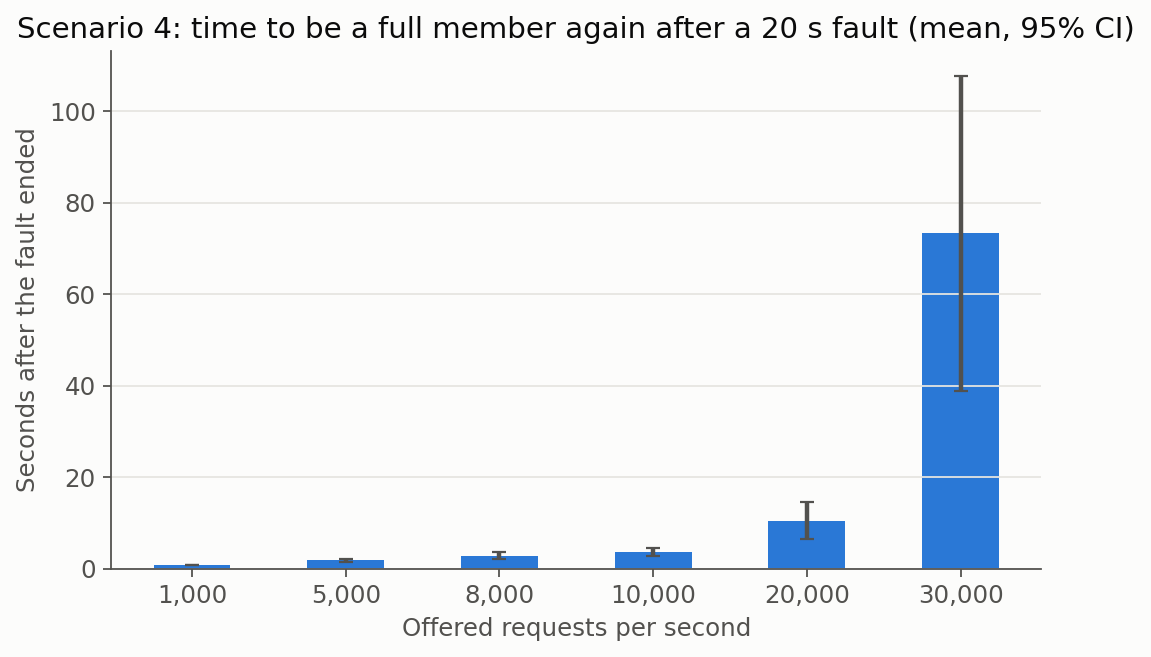
\includegraphics[width=0.78\linewidth]{figures/scenario4.png}
\caption{Scenario 4: time until the returning node was a member again, by load.}
\label{fig:s4}
\end{figure}

Recovery takes longer as load rises, because the node replays what it missed while new commands keep arriving: 0.8 s at 1,000 a second, 3.6 s at 10,000 and 10.5 s at 20,000. At 30,000 it took 73 s on average, most likely because little capacity is left on the air to catch up with. A shorter fault is quicker: 1.4 s after a 5 s fault at 10,000 a second, against 3.6 s after a 20 s one. A killed process has nothing in memory and rebuilds everything, in 6 s at 5,000 a second and 12 s at 10,000. Every run ended with one digest on all three nodes, within about 2 s of the load ending on average, and no checkpoint ever differed.

\textbf{Faults the nodes elect themselves.} With the fault election running every 20 to 30 s for 5 minutes at 3,000 a second, 5 runs gave 47 elected faults and 4,720,275 requests, with nobody giving up and 0 mismatches in 4,911 checkpoints. Over the 47 faults, the others dropped the silent node in a median of 1,018 ms (at most 1,036 ms), and it caught up with the log in a median of 428 ms after its silence ended (at most 1,141 ms).

\subsection{Two and three nodes killed}
\label{sec:kills}

This goes beyond one failure at a time, on the final build. Each run is 90 s with 10 s of warm-up, and both the nodes and the times are random: the first kill comes 15 to 30 s in, nodes stay down 5 to 20 s, and the last return leaves at least 25 s to recover. After each run, a checking tool lists what each node's own file applied, and every answer a client got is looked for there. Table~\ref{tab:kills} gives the cases at 10,000 reports a second with planning, the system's target load. The same cases were also run at 300, 15,000 and 20,000 a second.

\begin{table}[!htb]
\centering\small
\caption{Kills at 10,000 reports a second with planning, 3 runs per case, on the final build. Ranges are the lowest and highest run. Every case had 0 unaccounted and 0 digest mismatches.}
\label{tab:kills}
\begin{tabularx}{\linewidth}{@{}LrrP{2.6cm}P{2.0cm}P{2.0cm}@{}}
\toprule
Case & Answers/s & Answered & Gave up per run & Longest with no answer & Longest with no commit \\
\midrule
One node & 10,000 & 100.0\% & 0 & 0.9 to 1.0 s & 0.9 to 1.0 s \\
Two; first killed returns first & 9,848 & 96.7 to 99.6\% & 3,234 to 29,895 & 1.0 to 3.7 s & 1.6 to 8.7 s \\
Two; last killed returns first & 9,778 & 96.5 to 100.0\% & 0 to 31,219 & 1.4 to 1.9 s & 1.4 to 9.1 s \\
Two at the same moment & 9,555 & 93.2 to 97.3\% & 23,978 to 61,240 & 1.3 to 1.4 s & 8.1 to 10.9 s \\
Second killed just after first returns & 10,000 & 100.0\% & 0 & 1.0 s & 1.0 s \\
All three, back together & 9,197 & 86.4 to 97.3\% & 24,639 to 121,952 & 8.6 to 21.4 s & 8.6 to 21.4 s \\
All three, back one at a time & 8,567 & 83.3 to 87.5\% & 112,501 to 150,689 & 11.4 to 19.4 s & 11.4 to 19.4 s \\
\bottomrule
\end{tabularx}
\end{table}

Figure~\ref{fig:bynodes} shows the shape of these runs: what the cloud delivered with three, two, one and no nodes up. With one node up, most answers are provisional, which is the lone node answering on its own; when all are down, the few answers left come from the moments of rejoining.

\begin{figure}[!htb]
\centering
\begin{tikzpicture}
\begin{axis}[
  ybar stacked, bar width=0.75cm, width=0.72\linewidth, height=5.6cm,
  ymin=0, ymax=11500, ylabel={answers per second},
  symbolic x coords={3 up, 2 up, 1 up, 0 up}, xtick=data,
  yticklabel style={/pgf/number format/fixed, /pgf/number format/1000 sep={,}, font=\scriptsize},
  xticklabel style={font=\small}, label style={font=\scriptsize},
  legend style={font=\scriptsize, at={(0.98,0.98)}, anchor=north east, draw=black!30},
  axis lines*=left, ymajorgrids, grid style={black!10}, enlarge x limits=0.18,
]
\addplot[fill=nodeblue!55, draw=black!50] coordinates {(3 up,10208) (2 up,8621) (1 up,441) (0 up,337)};
\addlegendentry{committed}
\addplot[fill=notefill!80!clientorange, draw=black!50] coordinates {(3 up,0) (2 up,363) (1 up,1534) (0 up,0)};
\addlegendentry{provisional}
\end{axis}
\end{tikzpicture}
\caption{Answers per second by how many nodes were up, in the kill runs at 10,000 a second with planning, on the final build: 44, 27, 12 and 6 stretches of at least 3 s. One node alone answers about 2,000 a second, a bit under the third of the capacity it holds; stretches with three up include working off the backlog.}
\label{fig:bynodes}
\end{figure}

\textbf{The lab guide's T1 and T2 on the final build}, with 300 users: T1, a node killed and back, answered all 81,647 reports with a median of 98 ms, and nobody gave up. T2, one node killed and one silenced so that one is left for all three client PCs, answered all reports in each of its 3 runs, with about 4,850 provisional answers per run and equal digests at the end.

\subsection{Scale and stress: scenario 9}
\label{sec:stress}

The offered rate was raised until the answers stopped keeping up, with two planning loads: planning work 0, which tests what the protocol and the network can carry, and planning work 1000, about 4 ms of planning per report, which gives the real computing load the spec requires. Each run is 75 s, of which 60 s are measured, 5 runs per rate. A run ``held'' if it answered at least 99\% of the offered rate, nobody gave up, and p99 stayed under 3 s. This test is the team's own, not a requirement; 3 s allows an answer that needed the client's 2 s retry.

\begin{table}[!htb]
\centering\small
\caption{The stress series, mean of 5 runs. Cores is the mean CPU use per node.}
\label{tab:stress}
\begin{tabular}{@{}rrcrrrrrr@{}}
\toprule
Offered/s & Planning work & Held & Answered/s & Gave up & p50 ms & p95 ms & p99 ms & Cores \\
\midrule
5,000 & 0 & 5 of 5 & 5,004 & 0 & 137 & 180 & 227 & 0.3 \\
10,000 & 0 & 5 of 5 & 9,994 & 0 & 146 & 206 & 268 & 0.5 \\
20,000 & 0 & 5 of 5 & 20,007 & 0 & 171 & 317 & 451 & 0.9 \\
30,000 & 0 & 5 of 5 & 30,020 & 0 & 218 & 427 & 631 & 1.4 \\
33,000 & 0 & 3 of 5 & 32,197 & 5 & 271 & 1,723 & 3,814 & 1.5 \\
35,000 & 0 & 3 of 5 & 34,215 & 1,799 & 482 & 3,763 & 6,552 & 1.6 \\
36,000 & 0 & 1 of 5 & 34,070 & 2,160 & 633 & 5,569 & 10,323 & 1.6 \\
\midrule
1,000 & 1000 & 5 of 5 & 999 & 0 & 130 & 160 & 213 & 1.1 \\
5,000 & 1000 & 5 of 5 & 5,004 & 0 & 141 & 182 & 232 & 5.4 \\
10,000 & 1000 & 5 of 5 & 9,999 & 0 & 160 & 226 & 349 & 13.1 \\
12,000 & 1000 & 5 of 5 & 11,995 & 0 & 173 & 310 & 391 & 16.8 \\
14,000 & 1000 & 0 of 5 & 13,705 & 60 & 803 & 1,887 & 3,964 & 20.2 \\
\bottomrule
\end{tabular}
\end{table}

\begin{figure}[!htb]
\centering
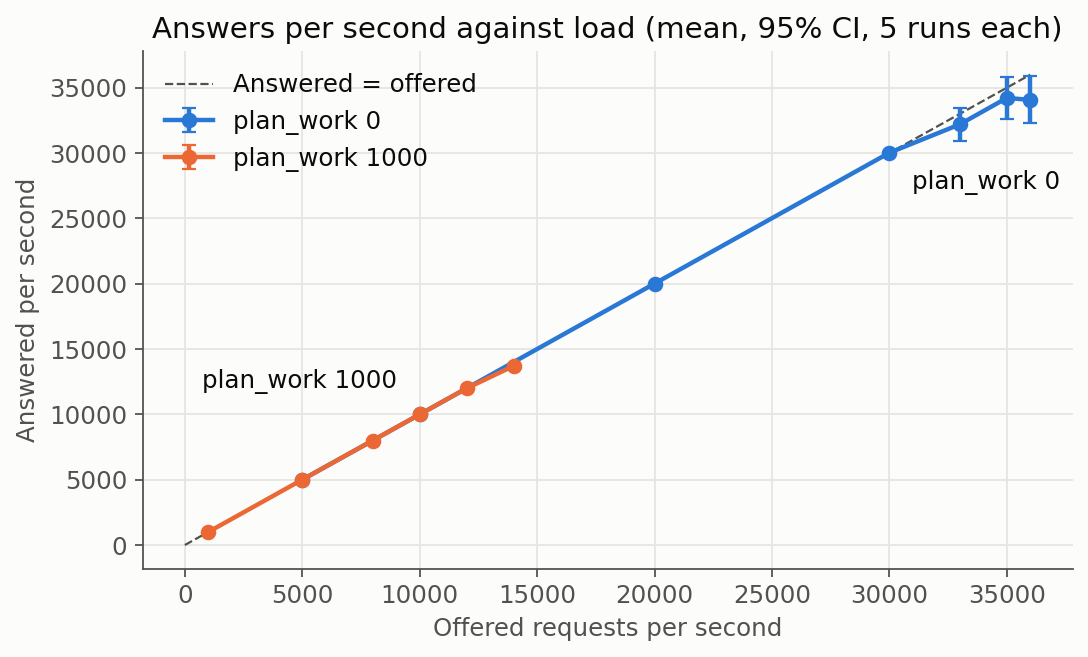
\includegraphics[width=0.49\linewidth]{figures/throughput.png}\hfill
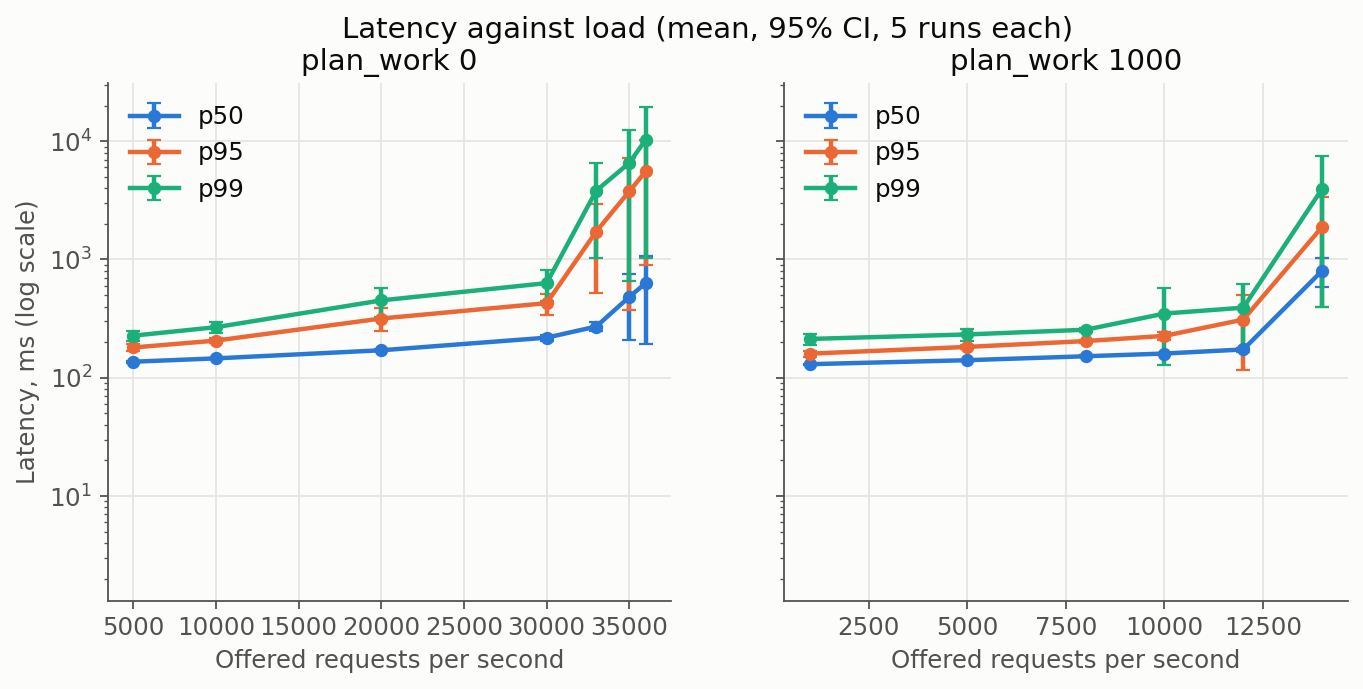
\includegraphics[width=0.49\linewidth]{figures/latency.png}
\caption{Throughput (left) and latency (right) against the offered rate, for both planning loads, mean of 5 runs.}
\label{fig:stress}
\end{figure}

\textbf{The ceiling} is 30,000 reports a second with almost no planning, held in all 5 runs and in a 5-minute hold (9,449,055 requests, p99 562 ms), and 12,000 a second with the planning load, held in all 5 runs. Above 30,000, results depend on the run. Answers per second stop rising at about 34,000.

\textbf{What limits it.} With planning, it is the CPU: the cores used per node rise with the rate, to about 20 at 14,000 a second, which is the size of the planning pool. Without planning, each node used under 2 cores above 30,000 a second, while elections saw fewer bids and retries rose. Fewer and smaller packets moved the ceiling up, which also points at the shared Wi-Fi. Air time was not measured directly.

\textbf{Where the time goes.} Latency is measured by the client, from when a report was due to go. Most of the median is the 60 ms election window, then the shared log. A p99 just over 2,000 ms means some answers needed the 2 s retry.

\textbf{Clients scale too.} The same 10,000 reports a second from one, two or three client PCs gave the same answered rate, with medians of 120, 130 and 146 ms, so the client PCs were not the limit. On the final build, 333 and 1,000 simulated users per client PC (999 and 3,000 in all, closed loop) answered every report.

\textbf{On a busier network.} At midday on November 5 the network was much busier. The final build answered all of 10,000 and 15,000 reports a second in 3 of 3 runs each, but at 30,000 it answered only 25,160 to 26,046 a second. To see whether the build or the network caused this, the overnight build was run again at midday at 30,000 a second, and it fell the same way. So 30,000 and above need a stable network, and the failure results are reported at 10,000 and 15,000.
